%\documentclass[11pt]{article}
\documentclass[11pt]{report}

\usepackage{amsmath,amssymb}
\usepackage{newcent}
\usepackage{pstricks} 
\usepackage{fancyhdr}
\usepackage[dvips]{graphicx}
\usepackage{makeidx}
\usepackage{psfrag}
\usepackage{alltt}
\usepackage{index}
\usepackage{fancyvrb}
\usepackage{pst-blur}
\usepackage{pst-grad}
\usepackage{epsfig}
%\usepackage{subfig}
\usepackage{subfigure}


\usepackage[colorlinks=true,linktocpage=true]{hyperref}

%% Listings package START
\usepackage{color}
\usepackage{listings}

\definecolor{darkblue}{rgb}{0,0,.6}
\definecolor{darkred}{rgb}{.6,0,0}
\definecolor{darkgreen}{rgb}{0,.6,0}
\definecolor{red}{rgb}{.98,0,0}
\definecolor{lightgrey}{rgb}{0.98,0.98,0.98}


\lstloadlanguages{C++}
\lstset{%
  language=C++,
  basicstyle=\small\ttfamily,
  commentstyle=\itshape\color{darkgreen},
  keywordstyle=\bfseries\color{darkblue},
  stringstyle=\color{darkred},
  showspaces=false,
  showtabs=false,
  columns=fixed,
  backgroundcolor=\color{lightgrey},
  numbers=none,
  frame=single,
  numberstyle=\tiny,
  breaklines=true,
  showstringspaces=false,
  xleftmargin=0.1cm
}%
%% Listings package STOP

%Keywords and Setup
\newcommand{\CMake} {\texttt{CMake}}
\newcommand{\OpenMP} {\texttt{OpenMP}}
\newcommand{\OpenCL} {\texttt{OpenCL}}
\newcommand{\ViennaCL} {\texttt{ViennaCL}}
\newcommand{\ViennaCLversion} {\texttt{ViennaCL 1.0.2}}
\newcommand{\ViennaCLminorversion} {\texttt{ViennaCL 1.0.x}}
\newcommand{\Boost} {\texttt{Boost}}
\newcommand{\ublas} {\texttt{ublas}}
\newcommand{\GCC} {\texttt{GCC}}
\newcommand{\MATLAB} {\texttt{MATLAB}}

% -*- mode: LaTeX -*-
% $Id: keywords.tex,v 1.6 2006/03/22 12:48:58 entner Exp $

% Specific text elements
\newcommand{\specific}[1] {\textit{#1}}
\newcommand{\extension}[1] {\textit{.#1}}
\newcommand{\email}[1]     {#1}

% Keywords and Indexing
%%%%%%%%%%%%%%%%%%%%%%%

% Enter keyword into keyword index
\newcommand{\keywordidx}[1]  {\index[idxkey]{#1@\texttt{#1}}}

% Print keyword within paragraph
\newcommand{\keyword}[1]     {\texttt{#1}}

% Print keyword and enter to keyword index
\newcommand{\keywordI}[1]    {\texttt{#1}{\keywordidx{#1}}}

% Print material parameter and enter to the mat.par.index
\newcommand{\ipdkeywordI}[1] {\texttt{#1}{\index[idxipd]{#1@\texttt{#1}}}}

% Print bold keyword and enter to the keyword index
%\newcommand{\bold}[1]        {{\bf \hyperpage{#1}}}
\newcommand{\keywordIB}[1]   {\texttt{#1}{\keywordidx{#1}}}

% Enter bold keyword to general index
\newcommand{\indexbold}[1]   {\index{#1|bold}}

% Print keyword and add to a second keyword in the keyword index:
\newcommand{\keywordII}[2]   {\texttt{#2}{\index[idxkey]{#1@\texttt{#2}}}}

% Environments for the model
%%%%%%%%%%%%%%%%%%%%%%%%%%%%

\newcommand{\psin}[1] {\varphi_{\mathrm{#1}}}
\newcommand{\IR}[1]   {I^R_\mathrm{N_#1}(\psin{1},\psin{2})}
\newcommand{\rhs}[1]  {\mathrm{rhs[N_#1]}}
\newcommand{\Y}[2]    {\mathrm{Y[N_#1][N_#2]}}

\newcommand{\mdlalphachar}{\mbox{\mdltt{[a-zA-Z]}}}
\newcommand{\mdlextendchar}{\mbox{\mdltt{[a-zA-Z0-9\_{\mdlbackslash}]}}}

\newcommand{\MdlBool}{\mdltt{Mdl\-Bool}}
\newcommand{\MdlString}{\mdltt{Mdl\-String}}
\newcommand{\MmuMdlKeyword}{\mdltt{Mmu\-Mdl\-Key\-word}}
\newcommand{\MmuMdlKeywordList}{\mdltt{MmuMdlKeywordList}}

\newcommand{\mdlAliasedModel}{\mdlkeyw{AliasedModel}}
\newcommand{\mdlEnd}{\mdlkeyw{End}}
\newcommand{\mdlinclude}{\mdlkeyw{\#include}}
\newcommand{\mdlInstance}{\mdlkeyw{Instance}}
\newcommand{\mdlinstantiate}{\mdlkeyw{instantiate}}
\newcommand{\mdlInterface}{\mdlkeyw{Interface}}
\newcommand{\mdlLinkMap}{\mdlkeyw{LinkMap}}
\newcommand{\mdlLoadObjectLibrary}{\mdlkeyw{LoadObjectLibrary}}
\newcommand{\mdlLocal}{\mdlkeyw{Local}}
\newcommand{\mdlModel}{\mdlkeyw{Model}}
\newcommand{\mdlNewModel}{\mdlkeyw{New\-Model}}
\newcommand{\mdlParameter}{\mdlkeyw{Parameter}}
\newcommand{\mdlParameters}{\mdlkeyw{Parameters}}
\newcommand{\mdlAnyParameter}{\mdlkeyw{AnyParameter}}
\newcommand{\mdlSelect}{\mdlkeyw{Select}}
\newcommand{\mdlStatic}{\mdlkeyw{Static}}
\newcommand{\mdlbreak}{\mdlkeyw{break}}
\newcommand{\mdlcalc}{\mdlkeyw{calc}}
\newcommand{\mdlcall}{\mdlkeyw{call}}
\newcommand{\mdlconstruct}{\mdlkeyw{construct}}
\newcommand{\mdlcontinue}{\mdlkeyw{continue}}
\newcommand{\mdldestruct}{\mdlkeyw{destruct}}
\newcommand{\mdldo}{\mdlkeyw{do}}
\newcommand{\mdlelse}{\mdlkeyw{else}}
\newcommand{\mdlerrors}{\mdlkeyw{errors}}
\newcommand{\mdlevaluate}{\mdlkeyw{evaluate}}
\newcommand{\mdlfalse}{\mdlkeyw{false}}
\newcommand{\mdlfor}{\mdlkeyw{for}}
\newcommand{\mdlgenLibrary}{\mdlkeyw{genLibrary}}
\newcommand{\mdlif}{\mdlkeyw{if}}
\newcommand{\mdlinitialize}{\mdlkeyw{initialize}}
\newcommand{\mdllink}{\mdlkeyw{link}}
\newcommand{\mdllistModels}{\mdlkeyw{listModels}}
\newcommand{\mdlmdlLibraryName}{\mdlkeyw{mdlLibraryName}}
\newcommand{\mdlmethod}{\mdlkeyw{method}}
\newcommand{\mdlof}{\mdlkeyw{of}}
\newcommand{\mdlparser}{\mdlkeyw{parser}}
\newcommand{\mdlprivate}{\mdlkeyw{private}}
\newcommand{\mdlprotected}{\mdlkeyw{protected}}
\newcommand{\mdlquiet}{\mdlkeyw{quiet}}
\newcommand{\mdlreturn}{\mdlkeyw{return}}
\newcommand{\mdlscanner}{\mdlkeyw{scanner}}
\newcommand{\mdlset}{\mdlkeyw{set}}
\newcommand{\mdlto}{\mdlkeyw{to}}
\newcommand{\mdltrue}{\mdlkeyw{true}}
\newcommand{\mdlverbose}{\mdlkeyw{verbose}}
\newcommand{\mdlwhile}{\mdlkeyw{while}}
\newcommand{\mdlCompilerProject}{\mdlkeyw{CompilerProject}}
\newcommand{\mdlcompile}{\mdlkeyw{compile}}
\newcommand{\mdlInfo}{\mdlkeyw{Info}}
\newcommand{\mdlundef}{\mdlkeyw{undef}}

\newcommand{\mdlModelClassDefinitionExtensions}{\mdltt{MODEL\_CLASS\_DEF\-INIT\-ION\_EX\-TENS\-IONS}}
\newcommand{\mdlModelClassStdConstructor}{\mdltt{Model\-Class\-Std\-Con\-struc\-tor}}
\newcommand{\mdlModelClassStdDestructor}{\mdltt{Model\-Class\-Std\-De\-struc\-tor}}
\newcommand{\mdlModelClassStdDeclarations}{\mdltt{Model\-Class\-Std\-Dec\-larat\-ions}}
\newcommand{\mdlModelClassInitExtension}{\mdltt{MODEL\_\-CLASS\_\-INIT\_\-EXT\-ENSION}}

\newcommand{\MDLPREFIXSTRING}{\mdltt{MDL\-PRE\-FIX\-STRING}}
\newcommand{\Model}{\mdltt{Model}}
\newcommand{\Parameter}{\mdltt{Parameter}}
\newcommand{\Interface}{\mdltt{Interface}}
\newcommand{\mdlbackslash}{\ensuremath{\mathtt{\backslash}}}
\newcommand{\divop}{\mathop{\rm div}}
\newcommand{\gradop}{\mathop{\rm grad}}
\newcommand{\asinh}{\mathop{\rm asinh}}

\newcommand{\unix}{\progname{Unix}}
\newcommand{\windows}{\progname{Windows-NT}}

% Some derived tables
\newenvironment{fixedwidthtable}     [2] {\begin{mmnttable}  {|l|p{10cm}|} {#1}                                  {#2}}     {\end{mmnttable}}
\newenvironment{fixedwidthtablep}    [3] {\begin{mmnttable}  {|l|p{#3}|}   {#1}                                  {#2}}     {\end{mmnttable}}
\newenvironment{fixedwidthtableL}    [3] {\begin{mmnttableL} {|l|p{10cm}|} {#1}                                  {#2}{#3}} {\end{mmnttableL}}
\newenvironment{fixedwidthTablep}    [3] {\begin{mmntTable}  {|l|p{#3}|}   {#1}                                  {#2}}     {\end{mmntTable}}
\newenvironment{fixedwidthTableL}    [3] {\begin{mmntTableL} {|l|p{10cm}|} {#1}                                  {#2}{#3}} {\end{mmntTableL}}
                                     
\newenvironment{keydesctableII}      [1] {\begin{mmnttable}  {|l|p{10cm}|} {Keyword & Description}               {#1}}     {\end{mmnttable}}
\newenvironment{keydesctableIIL}     [2] {\begin{mmnttableL} {|l|p{10cm}|} {Keyword & Description}               {#1}{#2}} {\end{mmnttableL}}
\newenvironment{keydesctableIILp}    [3] {\begin{mmnttableL} {|l|p{#3}|}   {Keyword & Description}               {#1}{#2}} {\end{mmnttableL}}
\newenvironment{keydesctableIII}     [1] {\begin{mmnttable}  {|l|l|l|}     {Keyword & Type & Description}        {#1}}     {\end{mmnttable}}
\newenvironment{keydesctableIIIL}    [2] {\begin{mmnttableL} {|l|l|l|}     {Keyword & Type & Description}        {#1}{#2}} {\end{mmnttableL}}
\newenvironment{keydesctableIIILp}   [3] {\begin{mmnttableL} {|l|l|p{#3}|} {Keyword & Type & Description}        {#1}{#2}} {\end{mmnttableL}}
\newenvironment{keydesctableIV}      [1] {\begin{mmnttable}  {|l|l|l|l|}   {Keyword & Type & Description & Unit} {#1}}     {\end{mmnttable}}
\newenvironment{keydesctableIVL}     [2] {\begin{mmnttableL} {|l|l|l|l|}   {Keyword & Type & Description & Unit} {#1}{#2}} {\end{mmnttableL}}

\newenvironment{keydescTableII}      [1] {\begin{mmntTable}  {|l|p{10cm}|} {Keyword & Description}               {#1}}     {\end{mmntTable}}
\newenvironment{keydescTableIIL}     [2] {\begin{mmntTableL} {|l|p{10cm}|} {Keyword & Description}               {#1}{#2}} {\end{mmntTableL}}
\newenvironment{keydescTableIII}     [1] {\begin{mmntTable}  {|l|l|l|}     {Keyword & Type & Description}        {#1}}     {\end{mmntTable}}
\newenvironment{keydescTableIIIL}    [2] {\begin{mmntTableL} {|l|l|l|}     {Keyword & Type & Description}        {#1}{#2}} {\end{mmntTableL}}
\newenvironment{keydescTableIIILp}   [3] {\begin{mmntTableL} {|l|l|p{#3}|} {Keyword & Type & Description}        {#1}{#2}} {\end{mmntTableL}}
\newenvironment{keydescTableIV}      [1] {\begin{mmntTable}  {|l|l|l|l|}   {Keyword & Type & Description & Unit} {#1}}     {\end{mmntTable}}
\newenvironment{keydescTableIVL}     [2] {\begin{mmntTableL} {|l|l|l|l|}   {Keyword & Type & Description & Unit} {#1}{#2}} {\end{mmntTableL}}

\newenvironment{keytypetableII}      [1] {\begin{mmnttable}  {|l|l|}       {Keyword & Type}                      {#1}}     {\end{mmnttable}}
\newenvironment{keytypetableIIL}     [2] {\begin{mmnttableL} {|l|l|}       {Keyword & Type}                      {#1}{#2}} {\end{mmnttableL}}
                                     
\newenvironment{keyunittableI}       [1] {\begin{mmnttable}  {|l|l|l|}     {Keyword & Type & Unit}               {#1}}     {\end{mmnttable}}

\newenvironment{parameterdescrtable} [1] {\begin{mmnttable}  {|l|l|}       {Parameter & Description}             {#1}}     {\end{mmnttable}}
\newenvironment{parameterdescrtableL}[2] {\begin{mmnttableL} {|l|l|}       {Parameter & Description}             {#1}{#2}} {\end{mmnttableL}}

\newenvironment{symbolkeytableII}    [1] {\begin{mmnttable}  {|l|l|}       {Symbol & Keyword}                    {#1}}     {\end{mmnttable}}
\newenvironment{symbolkeytableIIL}   [2] {\begin{mmnttableL} {|l|l|}       {Symbol & Keyword}                    {#1}{#2}} {\end{mmnttableL}}
\newenvironment{symbolkeytableIII}   [1] {\begin{mmnttable}  {|l|l|l|}     {Symbol & Keyword & Type}             {#1}}     {\end{mmnttable}}
\newenvironment{symbolkeyTableIII}   [1] {\begin{mmntTable}  {|l|l|l|}     {Symbol & Keyword & Type}             {#1}}     {\end{mmntTable}}
\newenvironment{symbolkeytableIIIL}  [2] {\begin{mmnttableL} {|l|l|l|}     {Symbol & Keyword & Type}             {#1}{#2}} {\end{mmnttableL}}
\newenvironment{symbolkeytableIV}    [1] {\begin{mmnttable}  {|l|l|l|l|}   {Symbol & Keyword & Type & Unit}      {#1}}     {\end{mmnttable}}
\newenvironment{symbolkeyTableIV}    [1] {\begin{mmntTable}  {|l|l|l|l|}   {Symbol & Keyword & Type & Unit}      {#1}}     {\end{mmntTable}}
\newenvironment{symbolkeytableIVL}   [2] {\begin{mmnttableL} {|l|l|l|l|}   {Symbol & Keyword & Type & Unit}      {#1}{#2}} {\end{mmnttableL}}
\newenvironment{symbolkeytableV}     [1] {\begin{mmnttable}  {|l|l|l|}     {Symbol & Keyword & Type}             {#1}}     {\end{mmnttable}}

\newenvironment{valuekeytableIII}    [1] {\begin{mmnttable}  {|l|l|l|}     {Keyword & Type & Values}             {#1}}     {\end{mmnttable}}
\newenvironment{valuekeytableIIIL}   [2] {\begin{mmnttableL} {|l|l|l|}     {Keyword & Type & Values}             {#1}{#2}} {\end{mmnttableL}}


\newcommand{\gcc} {GCC}


% File name
\newcommand{\file}[1]    {\stdin{#1}}
\newcommand{\fileI}[1]   {\file{#1}\index{#1}}
\newcommand{\fileIB}[1] {{\file{#1}}{\index{#1|bold}}}

% Some frequently used program names
\newcommand{\progname}[1]{\textsc{#1}}

\newcommand{\alib}{\progname{Algorithm Library}}
\newcommand{\cgg}{\progname{Cgg}}
\newcommand{\cpp}{\progname{C++}}
\newcommand{\C}{\progname{c}}
\newcommand{\tcl} {\progname{Tcl}}
\newcommand{\perl} {\progname{Perl}}
\newcommand{\ANSI}{\progname{Ansi}}
\newcommand{\ansic}{\progname{Ansi~c}}
\newcommand{\ansicpp}{\progname{nsi~\cpp}}
\newcommand{\posix}{\progname{Posix}}
\newcommand{\STL}{\progname{Stl}}
\newcommand{\emacs}{\progname{Emacs}}
\newcommand{\geo}{\progname{Geo2ps}}
\newcommand{\geotops}{\progname{Geo2ps}}
\newcommand{\inp}{\progname{Inp}}
\newcommand{\make}{\progname{Make}}
\newcommand{\makedevice}{\progname{makedevice}}
\newcommand{\MDL}{\progname{Model Definition Language}}
\newcommand{\mdl}{\progname{Mdl}}
\newcommand{\mkdev}{\progname{Makedevice}}
\newcommand{\python}{\progname{Python}}
\newcommand{\xmgrace}{\progname{Xmgrace}}
\newcommand{\xcrv}{\progname{Xcrv}}
\newcommand{\minimos}{\progname{Minimos~6}}
\newcommand{\mmnt}{\progname{Minimos-NT}}
\newcommand{\mdlprog}{\mmnt}
\newcommand{\mmtont}{\progname{Mm62nt}}
\newcommand{\pbf}{\progname{Pbf}}
\newcommand{\pbfm}{\progname{Pbfm}}
\newcommand{\pif}{\progname{Pif}}
\newcommand{\pifcopy}{\progname{Pifcopy}}
\newcommand{\pifrm}{\progname{Pifrm}}
\newcommand{\pifmaid}{\progname{Pifmaid}}
\newcommand{\prost}{\progname{Prost2d}}
\newcommand{\punch}{\progname{Punch}}
\newcommand{\rul}{\progname{Rul}}
\newcommand{\Siesta}{\progname{Siesta}}
\newcommand{\sketch}{\progname{Sketch}}
\newcommand{\spice}{\progname{Spice}}
\newcommand{\splitseg}{\progname{Splitseg}}
\newcommand{\svg}{\progname{Svg}}
\newcommand{\svgtops}{\progname{Svg2ps}}
\newcommand{\tif}{\progname{Tif}}
\newcommand{\str}{\progname{Str}}
\newcommand{\devedit}{\progname{Devedit}}
\newcommand{\silvaco}{\progname{Silvaco}}
\newcommand{\iseToPif}{\progname{Ise2pif}}
\newcommand{\synopsys}{\progname{Synopsys}}
\newcommand{\tifwrap}{\progname{Tifwrap}}
\newcommand{\tiftopif}{\progname{Tif2pbf.sh}}
\newcommand{\tsuprem}{\progname{Tsuprem4}}
\newcommand{\athena}{\progname{Athena}}
\newcommand{\xpif}{\progname{Xpif2d}}
\newcommand{\xsvg}{\progname{Xsvg}}
\newcommand{\vmake}{\progname{Vmake}}
\newcommand{\eas}{\progname{Eas}}

\newcommand{\pai}{\progname{Pai}}
\newcommand{\PAI}{\progname{Pai}}
\newcommand{\vista}{\progname{Vista}}
\newcommand{\PBF}{\progname{Pbf}}
\newcommand{\PBL}{\progname{Pbl}}
\newcommand{\PLB}{\progname{Plb}}
\newcommand{\PAL}{\progname{Pal}}
\newcommand{\FORTRAN}{\progname{Fortran}}
\newcommand{\LISP}{\progname{Lisp}}
\newcommand{\PIL}{\progname{Pil}}
\newcommand{\PCL}{\progname{Pcl}}
\newcommand{\PFL}{\progname{Pfl}}
\newcommand{\UNFUG}{\progname{Unfug}}
\newcommand{\DIOS}{\progname{Dios}}
\newcommand{\bison}{\progname{Bison}}
\newcommand{\flex}{\progname{Flex}}

\newcommand{\ipl}{ViennaIPD}
\newcommand{\inputdeck} {ViennaIPD}
\newcommand{\Inputdeck} {ViennaIPD}
%\newcommand{\inputdeck} {input-deck} % word within a paragraph
%\newcommand{\Inputdeck} {Input-deck} % at the beginning of a paragraph
%\newcommand{\InputDeck} {Input-Deck} % in headings

\newcommand{\curve}     {\sc{Curve}}

% simulation modes
\newcommand{\sm}{\sc{Single-Mode}}
\newcommand{\mm}{\sc{Mixed-Mode}}
\newcommand{\MM}{\sc{Mixed-Mode}}
\newcommand{\DC}{\sc{dc}}
\newcommand{\AC}{\sc{ac}}
\newcommand{\DD}{\sc{dd}}
\newcommand{\HD}{\sc{hd}}

% Name of a person (e.g. Maxwell)
\newcommand{\persname}[1]{\textsl{#1}}

\newcommand{\srh}{\persname{Shockley-Read-Hall}}

\newcommand{\key}[1]{\texttt{<#1>}}
\newcommand{\menu}[1]{\textsf{#1}}
\newcommand{\window}[1]{\textsl{\textsf{#1}}}

% Differential Operators: grad, div, rot, error function
\newcommand{\GRAD}{\mathrm{grad}}
\newcommand{\DIV}{\mathrm{div}}
\newcommand{\ROT}{\mathrm{rot}}
\newcommand{\erfc}{\mathrm{erfc}}

% Partial Derivative
\newcommand{\PD}[2]{\frac{\partial #1}{\partial #2}}

% Total Derivative
\newcommand{\TD}[2]{\frac{{\mathrm{d}} #1}{{\mathrm{d}} #2}}

% References to Equations, Tables, Figures, Sections
\newcommand{\Eq}[1]{(\ref{#1})}
\newcommand{\Fig}[1]{Fig.~\ref{#1}}
\newcommand{\Sec}[1]{Section~\ref{#1}}
\newcommand{\Chapter}[1]{Chapter~\ref{#1}}
\newcommand{\Appendix}[1]{Appendix~\ref{#1}}
\newcommand{\Table}[1]{Table~\ref{#1}}

% Vector
\newcommand{\vect}[1]{\mathbf{#1}}

% Bernoulli function
\newcommand{\bern}{\mathrm{B}}

% average D
\newcommand{\dav}{\overline{D}}

\newcommand{\ToKmO}{\left(\frac{\TL}{\mathrm{300\ K}} - 1\right)}
\newcommand{\ToK}{\left(\frac{\TL}{\mathrm{300\ K}}\right)}
\newcommand{\LToK}{\left(\frac{\TL}{\mathrm{77\ K}}\right)}
\newcommand{\LToKTH}{\left(\frac{\TL}{\mathrm{300\ K}}\right)}
\newcommand{\TK}{\left(\frac{T}{K}\right)}
\newcommand{\KoT}{\left(\frac{\mathrm{300\ K}}{\TL}\right)}
\newcommand{\KoLT}{\left(\frac{\mathrm{77\ K}}{\TL}\right)}

\newcommand{\dop}[2]      {\ensuremath{#1\times 10^{#2} \, \textrm{cm}^{-3}}}
\newcommand{\dopOne}[1]   {\ensuremath{10^{#1} \, \textrm{cm}^{-3}}}

\newcommand{\kL}      {\ensuremath{\kappa_\mathrm{L}}}

\newcommand{\nrg}  {\mathcal{E}}

\newcommand{\lth} {\lambda_\mathrm{TH}}
\newcommand{\hc}  {h_\mathrm{corr}}
\newcommand{\Qi}  {Q_\mathrm{i}}
\newcommand{\fB}  {f_\mathrm{B}}

\newcommand{\kdiel}   {\ensuremath{\kappa_\mathrm{diel}}}
\newcommand{\tdiel}   {\ensuremath{t_\mathrm{diel}}}
\newcommand{\mdiel}   {\ensuremath{m_\mathrm{diel}}}
\newcommand{\mOx}     {\ensuremath{m_\mathrm{ox}}}
\newcommand{\meff}    {\ensuremath{m_\mathrm{eff}}}
\newcommand{\kme}     {\ensuremath{\kappa_\mathrm{metal}}}
\newcommand{\ksi}     {\ensuremath{\kappa_\mathrm{si}}}
\newcommand{\epsr}[1]{\varepsilon_{\mathrm{r}}^{\mathrm{#1}}}
\newcommand{\q}{\mathrm{q}}
\newcommand{\kB}{\mathrm{k_B}}
\newcommand{\Ed}    {\nrg_\mathrm{d}}
\newcommand{\Ea}    {\nrg_\mathrm{a}}
\newcommand{\ED}    {\nrg_\mathrm{D}}
\newcommand{\EA}    {\nrg_\mathrm{A}}
\newcommand{\Ec}    {\nrg_\mathrm{C}}
\newcommand{\Eci}[1]{\nrg_\mathrm{C#1}}
\newcommand{\Ev}    {\nrg_\mathrm{V}}
\newcommand{\Evi}[1]{\nrg_\mathrm{V#1}}
\newcommand{\ET}    {\nrg_{\mathrm{T}}}
\newcommand{\rt}    {r_{\mathrm{t}}}
\newcommand{\ft}    {\ensuremath{f_{\mathrm{t}}}}
\newcommand{\Qt}    {\ensuremath{Q_{\mathrm{t}}}}
\newcommand{\Ei}    {\nrg_{\mathrm{i}}}
\newcommand{\Eref}  {\ensuremath{\nrg_{\mathrm{ref}}}}
\newcommand{\Ethr}  {\nrg_{\mathrm{thr}}}
\newcommand{\Eg}    {\nrg_{\mathrm{g}}}
\newcommand{\Egz}   {\nrg_{\mathrm{g,0}}}
\newcommand{\Eoff}  {\nrg_{\mathrm{off}}}
\newcommand{\GnII}{G_{n}^{\mathrm{II}}}
\newcommand{\GpII}{G_{p}^{\mathrm{II}}}
\newcommand{\NA}{N_\mathrm{A}}
\newcommand{\ND}{N_\mathrm{D}}
\newcommand{\Nc}{N_\mathrm{C}}
\newcommand{\Nv}{N_\mathrm{V}}
\newcommand{\Ncv}{N_\mathrm{C,V}}
\newcommand{\Ncz}{N_\mathrm{C,0}}
\newcommand{\Nvz}{N_\mathrm{V,0}}
\newcommand{\Ni}{N_{\mathrm{i}}}
\newcommand{\NT}{N_{\mathrm{T}}}
\newcommand{\Ntot}{N_{\mathrm{tot}}}
\newcommand{\TC}{T_{\mathrm{C}}}
\newcommand{\RDIR}{R^{\mathrm{DIR}}}
\newcommand{\RAU}{R^{\mathrm{AU}}}
\newcommand{\RBB}{R^{\mathrm{BB}}}
\newcommand{\RII}{R^{\mathrm{II}}}
\newcommand{\RSRH}{R^{\mathrm{SRH}}}
\newcommand{\RT}{R_{\mathrm{T}}}
\newcommand{\TL}{T_\mathrm{L}}
\newcommand{\TLo}{T_{L,\mathrm{old}}}
\newcommand{\tauen}{\tau_{\epsilon,n}}
\newcommand{\tauep}{\tau_{\epsilon,p}}
\newcommand{\taue}[1]{\tau_{\epsilon,#1}}
\newcommand{\TCoK}{\left(\frac{T_n}{\mathrm{300\ K}}+C_0\right)}
\newcommand{\PhiB}    {\ensuremath{\Phi_\mathrm{B}}}
\newcommand{\Phit}    {\ensuremath{\Phi_\mathrm{t}}}
\newcommand{\deriv}     {\ensuremath  {\mathrm{d}}}
\newcommand{\Schro}     {\persname{Schr{\"o}\-dinger}}

\newcommand{\Emin}      {\ensuremath{\nrg_\mathrm{min}}}
\newcommand{\Emax}      {\ensuremath{\nrg_\mathrm{max}}}
\newcommand{\Ef}        {\ensuremath{\nrg_\mathrm{F}}}
\newcommand{\Efi}       {\ensuremath{\nrg_{\mathrm{F},i}}}
\newcommand{\ef}[1]     {\ensuremath{\nrg_\mathrm{F#1}}}

\newcommand{\VEold}{\vect{E}_{\mathrm{old}}}
\newcommand{\VEoldi}[1]{\vect{E}_{\mathrm{old} #1}}
\newcommand{\VPold}{\vect{P}_{\mathrm{old}}}
\newcommand{\VPoldi}[1]{\vect{P}_{\mathrm{old} #1}}
\newcommand{\VP}[1]{\vect{P}_{#1}}
\newcommand{\Vg}        {\ensuremath{V_\mathrm{G}}}

\newcommand{\Iin}       {\ensuremath{I_\mathrm{in}}}
\newcommand{\Iout}      {\ensuremath{I_\mathrm{out}}}
\newcommand{\Vin}       {\ensuremath{V_\mathrm{in}}}
\newcommand{\Vout}      {\ensuremath{V_\mathrm{out}}}

\newcommand{\Vox}      {\ensuremath{V_\mathrm{ox}}}

\newcommand{\VDS}       {\ensuremath{V_\mathrm{DS}}}


\newcommand{\Id}        {\ensuremath{I_\mathrm{d}}}
\newcommand{\Vd}        {\ensuremath{V_\mathrm{d}}}
\newcommand{\Is}        {\ensuremath{I_\mathrm{s}}}

\newcommand{\te} {\ensuremath{\tau_\mathrm{e}}}
\newcommand{\tc} {\ensuremath{\tau_\mathrm{c}}}
\newcommand{\Nt} {\ensuremath{N_\mathrm{t}}}
\newcommand{\Et} {\ensuremath{\nrg_\mathrm{t}}}
\newcommand{\tox}{\ensuremath{t_\mathrm{ox}}}
\newcommand{\Di} {\ensuremath{D_\mathrm{i}}}

% install screen-shots

%% \newcommand{\leftpic}[3]{%
%%   \parpic[l]{%
%%   \psblurbox[linecolor=white,linewidth=0,framesep=-0.04,shadowsize=0.2cm,blurradius=0.1cm]{%
%%       \includegraphics[width=#1]{#2}} }  #3
%%   \picskip{0}
%%   \bigskip
%% }
%% \newcommand{\rightpic}[3]{%
%%   \parpic[r]{%
%%   \psblurbox[linecolor=white,linewidth=0,framesep=-0.04,shadowsize=0.2cm,blurradius=0.1cm]{%
%%       \includegraphics[width=#1]{#2}} }  #3
%%   \picskip{0}
%%   \bigskip
%% }

\newcommand{\leftpic}[3]{%
  \begin{minipage}{0.48\linewidth}
      \includegraphics[width=\linewidth]{#2}
  \end{minipage}
  \hfill
  \begin{minipage}{0.48\linewidth}
      #3
  \end{minipage}
}

\newcommand{\rightpic}[3]{%
  \begin{minipage}{0.48\linewidth}
      #3
  \end{minipage}
  \hfill
  \begin{minipage}{0.48\linewidth}
      \includegraphics[width=\linewidth]{#2}
  \end{minipage}
}

% makedevice
\newcommand{\SiO}{SiO$_2$}
\newcommand{\SiN}{Si$_3$N$_4$}


% abbreviations
\newcommand{\AIX}      {\sc Aix}
\newcommand{\ASCII}    {\sc Ascii}
\newcommand{\BICGSTAB} {\sc Bicg-stab}
\newcommand{\BJT}      {\sc Bjt}
\newcommand{\case}     {\sc Case}
\newcommand{\CNT}      {\sc Cnt}
\newcommand{\cpu}      {\sc Cpu}
\newcommand{\EEPROM}   {\sc Eeprom}
\newcommand{\EKV}      {\sc Ekv}
\newcommand{\FET}      {\sc Fet}
\newcommand{\GMRES}   {{\sc Gmres}(m)}
\newcommand{\HBT}      {\sc Hbt}
\newcommand{\HEMT}     {\sc Hemt}
\newcommand{\IBM}      {\sc Ibm}
\newcommand{\ILU}      {\sc Ilu}
\newcommand{\ILUFAC}   {Incomplete-{\LU} factorization}
\newcommand{\IUE}      {Institute for Microelectronics}
\newcommand{\LU}       {\sc Lu}
\newcommand{\MOS}      {\sc Mos}
\newcommand{\MOSFET}   {\sc Mosfet}
\newcommand{\NMOS}     {\sc Nmos}
\newcommand{\OSF}      {\sc Osf}
\newcommand{\PMOS}     {\sc Pmos}
\newcommand{\SOI}     {{\sc Soi}}
\newcommand{\SOIFET}   {\sc Soifet}
\newcommand{\TBB}      {\sc Tbb}
\newcommand{\TUV}      {Technical University Vienna}

\newcommand{\mydollar}   {\$} %$
\newcommand{\mytilde}    {{\ensuremath{{\sim}}}}

\newcommand{\MISSING}[1]{${}^*$\marginpar{${}^*$\textbf{Missing {#1}}}}

\newcommand{\NI}{${}^*$\marginpar{${}^*$\textbf{Not implemented!}}}

\newcommand{\BUG}{\marginpar{\includegraphics[width=1cm]{figures/bug.ps}}}

% Mobility functions
\newcommand{\mob}[1]{\mu^{\mathrm{#1}}}
\newcommand{\con}[1]{C^{\mathrm{#1}}}
\newcommand{\vs}{v^{\mathrm{sat}}}

\newcommand{\phis}[1]{\varphi_{\mathrm{s#1}}}
\newcommand{\psis} {\varphi_{\mathrm{s}}}
\newcommand{\psim} {\varphi_{\mathrm{m}}}
\newcommand{\psibi}{\psi_{\mathrm{bi}}}
\newcommand{\psiwf}{\varphi_{\mathrm{wf}}}
\newcommand{\psiox}{\varphi_{\mathrm{ins}}}
\newcommand{\psiqfl}{\varphi_{\mathrm{qfl}}}
\newcommand{\Ewf}{\nrg_{\mathrm{w}}}
\newcommand{\eps}[1]{\varepsilon_{\mathrm{#1}}}
\newcommand{\mL}{{\mathrm{L}}}

\newcommand{\qf}  {quasi-\persname{Fermi}} % is not coupled to index entries

\newcommand{\BB}   {\sc bb}
\newcommand{\BGN}  {\sc Bgn}
\newcommand{\BNF}  {\sc Bnf}
\newcommand{\CQFL} {\sc Cqfl}
\newcommand{\QTBM} {\sc Qtbm}
\newcommand{\WKB}  {\sc Wkb}
\newcommand{\TFE}  {\sc Tfe}
\newcommand{\TE}   {\sc Te}
\newcommand{\SI}   {\sc si}

\newcommand{\Nit}         {\ensuremath{N_\mathrm{it}}}
\newcommand{\Nz}          {\ensuremath{N_0}}
\newcommand{\kf}          {\ensuremath{k_\mathrm{f}}}
\newcommand{\kfz}         {\ensuremath{k_\mathrm{f,0}}}
\newcommand{\kr}          {\ensuremath{k_\mathrm{r}}}
\newcommand{\NXz}         {\ensuremath{N_{X,\mathrm{it}}}}
\newcommand{\ps}          {\ensuremath{p_\mathrm{s}}}
\newcommand{\Eox}         {\ensuremath{E_\mathrm{ox}}}
\newcommand{\pref}        {\ensuremath{p_\mathrm{ref}}}
\newcommand{\Qit}         {\ensuremath{Q_\mathrm{it}}}
\newcommand{\Qitsimple}   {\ensuremath{Q_\mathrm{it}^\mathrm{simple}}}
\newcommand{\Dt}          {\ensuremath{D_\mathrm{t}}}
\newcommand{\Qf}          {\ensuremath{Q_\mathrm{f}}}
\newcommand{\EF}          {E_{\mathrm{F}}}
\newcommand{\Vth}         {V_\mathrm{th}}
\newcommand{\Cox}         {\ensuremath{C_\mathrm{ox}}}
\newcommand{\NX}          {\ensuremath{N_X}}
\newcommand{\DX}          {\ensuremath{D_X}}
\newcommand{\DXz}         {\ensuremath{D_{X,0}}}
\newcommand{\PhiX}        {\ensuremath{\Phi_X}}

 % [KR] This is a mess, we should delete unused Minimos-stuff
% Define margins
\voffset=-1in
\hoffset=-1in

% A4
\headheight=4ex
\headsep=2ex

\evensidemargin=2.5cm
\oddsidemargin=2.5cm
%\topmargin=1.3cm
\topmargin=0.0cm
\marginparwidth=1.5cm

\textwidth=16.0cm
\textheight=23.9cm

\footskip=6ex
\parindent=0cm
\parskip=1ex

\newlength{\mmntboxwidth}
\setlength{\mmntboxwidth}{\textwidth}
\addtolength{\mmntboxwidth}{-2mm}

\setcounter{secnumdepth}{4}
\setcounter{tocdepth}{2}

\shortindexingoff
%\newindex{idxkey}{idxkey}{indkey}{Index of Keywords}
%\newindex{idxipd}{idxipd}{indipd}{Index of Material Parameters}
\makeindex

\newcommand{\auxindex}[1]{\index{auxiliary tools!#1@\texttt{#1}}%
\index{#1@\texttt{#1}}}

\newlength{\NoteBoxWidth}
\setlength{\NoteBoxWidth}{14.5cm}%{15.18cm}
\newrgbcolor{notebg}         {0.99609375 0.8828125 0.921875}  % PSTricks colors
\newrgbcolor{tipbg}          {0.98828125 0.99609375 0.78515625}
\newrgbcolor{ipdbg}          {0.85  0.85  0.93}
\definecolor{headingfg} {rgb}{0.2,0.2,0.6}
\newrgbcolor{headingfg}      {0.2 0.2 0.6}  % PSTricks colors

\newlength{\IpdBoxWidth}
\setlength{\IpdBoxWidth}{14.5cm}

\newcommand{\verbbaseformat}[2] {\psframebox*[boxsep=false,fillcolor=#1]{
                                 %\parbox{\IpdBoxWidth}{\color{black}#2\raisebox{-1ex}{\rule{0pt}{2.6ex}}}}}
                                 \parbox{\IpdBoxWidth}{\color{black}#2\raisebox{-1.5ex}{\rule{0pt}{2.6ex}}}}}
\newcommand{\verbformat}[1]     {\verbbaseformat{\verbatimbg}{#1}}
\newcommand{\verbatimbg}        {ipdbg}
\renewcommand{\FancyVerbFormatLine}[1]{\verbformat{#1}}

\newcommand{\EXA}{}
\newcommand{\mmntcaparg}{}
\newcommand{\mmntlabarg}{}
\newcommand{\stdin}[1]{\texttt{#1}}
\newcommand{\unit}[1]{$\mathrm{#1}$}

\makeatletter % [JW] check latex faq for : \@ and @ in macro names
\newcommand{\mmnttablecaption}[1]{%
\par
\addcontentsline{lot}{table}{\protect\numberline{thetable}{\ignorespaces #1}}
\refstepcounter{table}\@makecaption{\fnum@table}{#1\rule[-2mm]{0mm}{3mm}}}

\newcommand{\TIP}[1]{\vspace*{0.4cm}
\marginpar[{\vspace{0.1cm}\hspace{ 0.8cm}
\includegraphics[width=0.7cm]{figures/tip.eps}}]%
          {{\vspace{0.1cm}\hspace{-0.2cm}
\includegraphics[width=0.7cm]{figures/tip.eps}}}%
\hspace{0.5cm}\psframebox*[fillcolor=tipbg]{\parbox{\NoteBoxWidth}{#1}}\vspace*{0.4cm}}

\newcommand{\NOTE}[1]{\vspace*{0.4cm}
\marginpar[{\vspace{0.15cm}\hspace{ 0.8cm}
\includegraphics[width=0.7cm]{figures/note.eps}}]%
          {{\vspace{0.15cm}\hspace{-0.2cm}
\includegraphics[width=0.7cm]{figures/note.eps}}}%
\hspace{0.5cm}\psframebox*[fillcolor=notebg]{\parbox{\NoteBoxWidth}{#1}}\vspace*{0.4cm}}

\newcommand{\listitem} {\psframe[fillstyle=gradient,gradbegin=headingfg,gradend=headingfg,gradmidpoint=1,linestyle=none](-0.15,0.075)(0.0,0.225)}

\newenvironment{mmnttable}[3]
{\renewcommand{\mmntcaparg}{#3}\par\vspace{3mm}\begin{minipage}{\textwidth}
\begin{center}\par\begin{tabular}{#1} \hline #2 \\ \hline}
{\hline \end{tabular}\mmnttablecaption{\mmntcaparg}\end{center}\end{minipage}}
\makeatother

\newenvironment{exaipd}
{ %\begin{list}{}{\leftmargin6mm} \scriptsize\item[]\EXA }
 \begin{list}{}{\leftmargin6mm} \scriptsize\item[]\EXA }
{\end{list}}

\newenvironment{mmnttableL}[4]
{\renewcommand{\mmntcaparg}{#3}\renewcommand{\mmntlabarg}{#4}\par
\vspace{3mm}\begin{minipage}{\textwidth}\begin{center}\par\begin{tabular}{#1}
\hline #2 \\ \hline}
{\hline \end{tabular}\mmnttablecaption{\mmntcaparg}\label{\mmntlabarg}
\end{center}\end{minipage}}

\newenvironment{mmntlist}
{\par\vspace*{-0.1cm}%
  \begin{list}{\listitem}%
      {\setlength{\itemsep}{0.001cm}}%
}%
{\end{list}\vspace*{-0.1cm}}



\begin{document}
\pagenumbering{roman}


\begin{titlepage}

\vspace*{3cm}
\huge{MATLAB Interface} 
\rule[0.0cm]{9.3cm}{0.05cm}
\begin{flushright}
\Large{for ViennaCL 1.0.2}
%\Large{User Manual}
%\Large{Building Instructions}\\
%\Large{Input Specifications}
\end{flushright}

\vspace{13cm}
\rule[0.0cm]{16.0cm}{0.05cm}
\begin{figure}[!ht]
   \vspace{-1.0cm}
   \centering
   \begin{minipage}{3cm}
      
\epsfig{file=figures/TU_Signet_CMYK, scale=0.25}
   \end{minipage}
   \hfill
   \hspace{-0.5cm}
   \begin{minipage}{5.5cm}
      \vspace{0.5cm}
      \begin{center}
      Institute for Microelectronics\newline
      Gu\ss hausstra\ss e 27-29 / E360\newline 
      A-1040 Vienna, Austria\newline
      \end{center}
   \end{minipage}   
   \hfill   
   \begin{minipage}{2.6cm}
      
\epsfig{file=figures/logo_px200, scale=1.6}
   \end{minipage}
\end{figure}

\end{titlepage}



\clearpage

Copyright {\copyright} 2010, Institute for Microelectronics, TU Vienna.

\vspace{2.5cm}

Main Contributors:\\ 

Florian Rudolf\\
Karl Rupp\\
Josef Weinbub\\

\vspace{2.5cm}

Current Maintainers: \\

Florian Rudolf\\
Karl Rupp\\
Josef Weinbub\\


\vspace{7.0cm}

Institute for Microelectronics\newline
Vienna University of Technology\newline
Gu\ss hausstra\ss e 27-29 / E360\newline
A-1040 Vienna, Austria/Europe\newline


\begin{tabular}{ll}
Phone  & +43-1-58801-36001\\
FAX    & +43-1-58801-36099\\
Web    & \texttt{http://www.iue.tuwien.ac.at}
\end{tabular}





\clearpage

\addtocontents{toc}{\protect\setcounter{tocdepth}{1}} 
\tableofcontents
%\label{s:ipl:content} \index{IPL!content}

\clearpage
\pagenumbering{arabic}

\chapter*{Introduction}   \addcontentsline{toc}{chapter}{Introduction}

The MATLAB interface of {\ViennaCL} provides simple access to the computational resources of GPUs using {\ViennaCL} under MATLAB.
An interface for the following iterative solvers (confer for example to the book of Y.~Saad \cite{saad-iterative-solution}) is provided:
\begin{itemize}
 \item Conjugate Gradient (CG)
 \item Stabilized BiConjugate Gradient (BiCGStab)
 \item Generalized Minimum Residual (GMRES)
\end{itemize}
In the current version, all solvers are provided without preconditioner. Since MATLAB relies on double precision arithmetics, only a few GPUs can be used, see Tab.~\ref{tab:double-precision-GPUs}.

\NOTE{Double precision arithmetic on GPUs is only possible if it is provided by the GPU. There is no double precision emulation in {\ViennaCL}.}

\begin{table}[tb]
\begin{center}
\begin{tabular}{l|c}
Compute Device & ViennaCL-Matlab \\
\hline
Nvidia Geforce 86XX GT/GSO   & no \\
Nvidia Geforce 88XX GTX/GTS  & no \\
Nvidia Geforce 96XX GT/GSO   & no \\
Nvidia Geforce 98XX GTX/GTS  & no \\
Nvidia GT 230     & no \\
Nvidia GT(S) 240  & no \\
Nvidia GTS 250    & no \\
Nvidia GTX 260    & yes \\
Nvidia GTX 275    & yes \\
Nvidia GTX 280    & yes \\
Nvidia GTX 285    & yes \\
Nvidia GTX 465    & yes \\
Nvidia GTX 470    & yes \\
Nvidia GTX 480    & yes \\
Nvidia Quadro FX 46XX & no \\
Nvidia Quadro FX 48XX & yes \\
Nvidia Quadro FX 56XX & no \\
Nvidia Quadro FX 58XX & yes \\
Nvidia Tesla 870    & no \\
Nvidia Tesla C10XX  & yes \\
Nvidia Tesla C20XX  & yes \\
\hline
ATI Radeon HD 45XX   & no \\
ATI Radeon HD 46XX   & no \\
ATI Radeon HD 47XX   & no \\
ATI Radeon HD 48XX   & maybe \\
ATI Radeon HD 54XX   & no \\
ATI Radeon HD 55XX   & no \\
ATI Radeon HD 56XX   & no \\
ATI Radeon HD 57XX   & no \\
ATI Radeon HD 58XX   & maybe \\
ATI Radeon HD 59XX   & maybe \\
ATI FireStream V92XX & maybe \\
ATI FirePro V78XX    & maybe \\
ATI FirePro V87XX    & maybe \\
ATI FirePro V88XX    & maybe \\
\end{tabular}
\caption{Supported GPUs for the MATLAB interface of {\ViennaCL}. At the release of the MATLAB interface for {\ViennaCLversion}, GPUs from AMD/ATI do not comply to {\OpenCL} standard for double precision extensions. Once the driver of these GPUs complies to the double precision extension standard of {\OpenCL}, they can be used with the MATLAB interface for {\ViennaCL} immediately.}
\label{tab:double-precision-GPUs}
\end{center}
\end{table}

\chapter{Installation and Usage}
%The good news at the beginning of this chapter is that 
%{\ViennaCL} is a header-only library. Therefore, you do NOT have to build any static or shared
%libraries, copy them to the correct place and set linker paths appropriately
%In fact, all you have to do is copy the folder \lstinline|viennacl/| either to
%the global system include path or directly into your project directory.

This chapter shows how the {\MATLAB} interface for {\ViennaCL} is compiled and how it can be used. The necessary steps are outlined for several different platforms, but we could not check every possible combination of hardware, operating system and compiler. If you experience any trouble, please write to the maining list at \\
\begin{center}
\texttt{viennacl-support$@$lists.sourceforge.net} 
\end{center}


% -----------------------------------------------------------------------------
% -----------------------------------------------------------------------------
\section{Dependencies}
% -----------------------------------------------------------------------------
% -----------------------------------------------------------------------------
\label{dependencies}

\begin{itemize}
 \item A {\MATLAB} version with MEX-interface (eg.~R2009a)
 \item A recent C++ compiler (~{\GCC} \texttt{4.2.x} and higher as well as the \texttt{Visual C++} compiler in Visual Studio 2008 are known to work)
 \item {\OpenCL}~\cite{khronoscl,nvidiacl} for accessing compute devices (GPUs);
see Section~\ref{opencllibs} for details.
\end{itemize}

% -----------------------------------------------------------------------------
% -----------------------------------------------------------------------------
\section{Get the {\OpenCL} Library}
\label{opencllibs}
% -----------------------------------------------------------------------------
% -----------------------------------------------------------------------------
The development of {\OpenCL} applications based on graphics cards 
requires a suitable driver and a corresponding library, e.g.~\texttt{libOpenCL.so} under Unix based systems.
This section describes how this library can be acquired.

\TIP{Note, that for Mac OS X systems there is no need to install an {\OpenCL} 
capable driver and the corresponding library. 
The {\OpenCL} library is already present if a suitable graphics 
card is present. Using {\ViennaCL} on Mac OS X is discussed in Section~\ref{apple}.}				

\subsection{NVIDIA cards}
NVIDIA provides the {\OpenCL} library with the driver. Therefore, if a 
NVIDIA driver is present on the system, the library is too. However, 
not all of the released drivers contain the {\OpenCL} library. 
A driver which is known to support {\OpenCL}, and hence providing the required
library, is $195.36.24$. 

\subsection{ATI cards}
As of the release of {\ViennaCL}, ATI cards lack the ability of full 
double support~\cite{atidouble}. Since the {\MATLAB} interface for {\ViennaCL} requires double precision support,
it cannot be used unless full standard-compliant double precision support is made available from AMD/ATI.

% -----------------------------------------------------------------------------
% -----------------------------------------------------------------------------
\section{Building the {\MATLAB} Interface}
% -----------------------------------------------------------------------------
% -----------------------------------------------------------------------------

In the following a generic description is given, then some OS-specific details are explained.

The first step is to configure {\MATLAB}. Type
\begin{lstlisting}
 mex -setup
\end{lstlisting}
and choose a suitable C++ compiler.

\TIP{Make sure that the selected compiler supports C++, not just C.}

Then change into the base directory of the {\MATLAB} interface for {\ViennaCL}. If the {\OpenCL} include and library files are installed system-wide, the commands
\begin{lstlisting}
 mex viennacl_cg.cpp       -I. -lOpenCL
 mex viennacl_bicgstab.cpp -I. -lOpenCL
 mex viennacl_gmres.cpp    -I. -lOpenCL
\end{lstlisting}
build the three solvers.

\NOTE{On 64-bit systems, you may have to append the \texttt{-largeArrayDims} option, otherwise you might get a runtime error when calling the solvers.}

\subsection{Linux}
If you are using a new version of \GCC (4.3.x and above), you may get linker errors when calling any of the solvers. In that case, install version 4.2 of {\GCC} and change the compiler call in 
\begin{center}\texttt{\${HOME}/.matlab/{{\MATLAB}VERSION}/mexopts.sh} \end{center}
to e.g.~\texttt{g++-4.2}, where \texttt{{\MATLAB}VERSION} refers to you {\MATLAB} version, e.g.~\texttt{R2010a}.

\TIP{On Ubuntu, you can directly install \GCC in version 4.2.x from the repository. The executeable is called \texttt{g++-4.2}.}

\subsection{Mac OS X}
\label{apple}
The tools mentioned in Section \ref{dependencies} are available on 
macintosh platforms too. 
For the {\GCC} compiler the Xcode~\cite{xcode} package has to be installed.
To install {\CMake} and {\Boost} external portation tools have to be used, 
for example, Fink~\cite{fink}, DarwinPorts~\cite{darwinports} 
or MacPorts~\cite{macports}. Such portation tools provide the 
aforementioned packages, {\CMake} and {\Boost}, for macintosh platforms. 

For Mac OS X, the following linker flag has to be added to the compilation call.
\begin{lstlisting}
 -framework OpenCL
\end{lstlisting}
This is best done in the \text{mexopts.sh} file usually located at
\begin{center}\texttt{\${HOME}/.matlab/{{\MATLAB}VERSION}/mexopts.sh} . \end{center}
Typically, this is achieved by adding
\begin{lstlisting}
 -framework OpenCL
\end{lstlisting}
to the C++ compiler flags \texttt{CXXFLAGS} for your architecture (mind that the configuration for both 32 bit and 64 bit systems is located in the mexopts file).

\subsection{Windows}
Since the include and library files for {\OpenCL} are usually not available system-wide, you have to specify their location manually. Assuming that the NVidia CUDA SDK located at \texttt{C:$\setminus$CUDA$\setminus$} is used, type
\begin{lstlisting}
 mex viennacl_cg.cpp       -I. -IC:\CUDA\include -LC:\CUDA\lib -lOpenCL
 mex viennacl_bicgstab.cpp -I. -IC:\CUDA\include -LC:\CUDA\lib -lOpenCL
 mex viennacl_gmres.cpp    -I. -IC:\CUDA\include -LC:\CUDA\lib -lOpenCL
\end{lstlisting}


\section{Usage} \label{sec:usage}
Simply call the {\ViennaCL} solver interface as for the built-in functions provided by {\MATLAB}:
\begin{lstlisting}
 result = viennacl_cg(A, rhs);
 result = viennacl_bicgstab(A, rhs);
 result = viennacl_gmres(A, rhs);
\end{lstlisting}

There are a few things to note about the performance of the solvers provided by {\ViennaCL}:
\begin{itemize}
 \item At the very first invocation of a {\ViennaCL}, the {\OpenCL} compute kernels are compiled, which may take a few seconds. Subsequent calls of any {\ViennaCL} solvers do not have this overhead.
 \item Since {\MATLAB} stores sparse matrices column-wise, but {\ViennaCL} requires a row-wise storage, the non-symmetric system matrices for \texttt{BiCGStab} and \texttt{GMRES} have to be rearranged in system memory.
 \item On 32-bit systems, matrix indices are stored as \texttt{signed integers}, whereas {\ViennaCL} requires \texttt{unsigned integers}. Thus, the data structures holding the matrix indices have to be converted, which is also a runtime penalty. At present, indices are also converted on 64-bit systems, even if this may not be required.
 \item All data has to be transferred to the GPU before the solver can start.
 \item The solution vector needs to be copied from the GPU back to the main memory, which also constitutes a runtime penalty.
\end{itemize}
Therefore, the use of the {\ViennaCL} solvers in {\MATLAB} does not pay off for small systems with only a few unknowns (say, less than $10.000$) and very well conditioned systems which need only a few solver iterations to converge. The general rule of thumb is that at least twenty to forty iterations are required to have a significant benefit using {\ViennaCL}, cf.~Chap.~\ref{chap:benchmarks}.



\chapter{Benchmark Results}\label{chap:benchmarks}
We have compared the performance of the conjugate gradient solver provided via the {\MATLAB} interface of {\ViennaCL} with the built-in functions of {\MATLAB}. The code used for the benchmarks can be found in the files \texttt{test\_cg.m}.

\begin{center}
\begin{tabular}{|l|l|}
\hline
CPU & Intel Core i7 960 \\
GPU & NVidia Geforce GTX 470 \\
RAM & 6 GB \\
OS  & Windows 7 Ultimate, 32 bit \\
Nvidia driver version: & 197.75 \\
{\ViennaCL} version  & 1.0.2 \\
\hline
\end{tabular}
\end{center}

\NOTE{Compute kernels are not fully optimized yet, results are likely to improve considerably in future releases of {\ViennaCL}}

\begin{figure}[tbp]
    \centerline{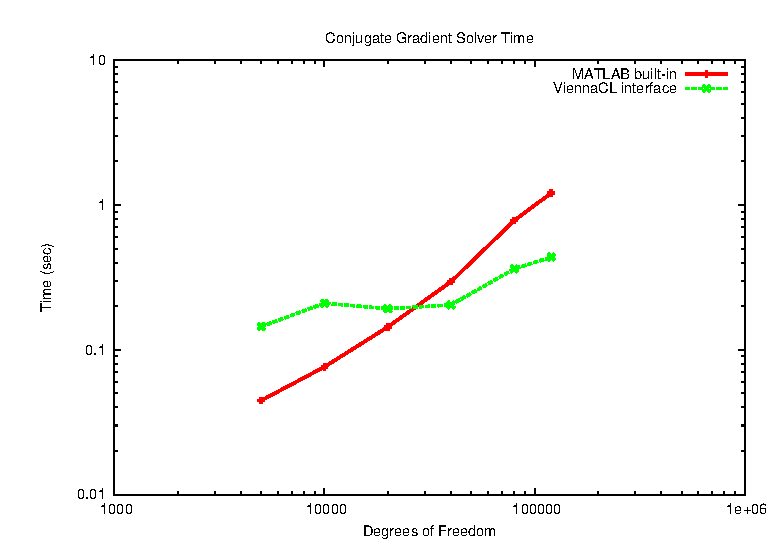
\includegraphics[width=0.9\textwidth]{figures/cg-matlab}}
    \caption{Execution time for ten conjugate gradient solver runs (27 iterations each) for different problem sizes. }
    \label{fig:matlab-cg}
\end{figure}

The results in Fig.~\ref{fig:matlab-cg} show that there is a certain overhead related to starting the compute kernels in {\OpenCL}. However, for large systems, this overhead becomes negligible and the performance benefit can readily be seen. 

\chapter*{Change Logs} \addcontentsline{toc}{chapter}{Change Logs}

\section*{Version 1.0.x}
\subsection*{Version 1.0.2} 
First release of the MATLAB interface for {\ViennaCL}.


\chapter*{License}  \addcontentsline{toc}{chapter}{License}

Copyright (c) 2010, Institute for Microelectronics, TU Wien

Permission is hereby granted, free of charge, to any person obtaining a copy
of this software and associated documentation files (the "Software"), to deal
in the Software without restriction, including without limitation the rights
to use, copy, modify, merge, publish, distribute, sublicense, and/or sell
copies of the Software, and to permit persons to whom the Software is
furnished to do so, subject to the following conditions:

The above copyright notice and this permission notice shall be included in
all copies or substantial portions of the Software.

THE SOFTWARE IS PROVIDED "AS IS", WITHOUT WARRANTY OF ANY KIND, EXPRESS OR
IMPLIED, INCLUDING BUT NOT LIMITED TO THE WARRANTIES OF MERCHANTABILITY,
FITNESS FOR A PARTICULAR PURPOSE AND NONINFRINGEMENT. IN NO EVENT SHALL THE
AUTHORS OR COPYRIGHT HOLDERS BE LIABLE FOR ANY CLAIM, DAMAGES OR OTHER
LIABILITY, WHETHER IN AN ACTION OF CONTRACT, TORT OR OTHERWISE, ARISING FROM,
OUT OF OR IN CONNECTION WITH THE SOFTWARE OR THE USE OR OTHER DEALINGS IN
THE SOFTWARE.

%\section{Bibliography}
\bibliographystyle{IEEEtran_v1.13}
\addcontentsline{toc}{chapter}{Bibliography} 
\bibliography{viennacl}

%\cleardoublepage
%\phantomsection
%\addcontentsline{toc}{chapter}{Index}
\printindex

\end{document}
